\section{Evaluation}
\label{sec:evaluation}

In this section, we describe an evaluation of \toolname{} on a set of Rust benchmarks.

\paragraph{Benchmarks}
We evaluate \toolname{} on a benchmark set comprising eleven Rust data structure modules drawn from the Verus GitHub repository~\cite{verus} as well as other open-source repositories.
A list of the benchmarks is shown in \Cref{tab:benchmarks}.
Although the original sources are publicly available, our benchmarks have been substantially modified with more complete specifications, additional methods, and unit tests. We verified that the versions used in our evaluation do not appear verbatim in the \texttt{o1-2024-12-17} training snapshot; for example, no form of our fully verified \textsc{RingBuffer} appears in the dataset. Furthermore, even if older versions existed in pretraining data, our baseline results demonstrate that LLMs still struggle to synthesize correct Verus specifications without structured guidance---underscoring the necessity of \toolname{}'s workflow.
The benchmarks cover a set of commonly-used data structures, including a ring buffer, a vector implementation with set abstractions and common algorithms, a polymorphic option type, tree-based modules for standalone nodes and a treemap, a bitmap with 64-bit blocks, and concurrent data structures such as a read–write lock and an invariant framework for shared state. Each benchmark contains 5--21 functions to verify, where the number of functions refers to the total number of member methods in the data structure module and the corresponding test functions. In total, our benchmark set includes 129 functions to be verified across all modules. 

\begin{table*}[t]
  % \vspace*{-7.9em}

\caption{Benchmark set consisting of eleven data structures.}
\label{tab:benchmarks}
\begin{small}
\begin{tabular}{|c|p{7.8cm}|c|}
\hline
\textbf{Benchmark} & \textbf{Description} & \textbf{\#Functions} \\
\hline
\textsc{Atomics} & An atomic counter in concurrent programming. & 11 \\
\hline
\textsc{Bitmap} & Bitmap implemented over 64-bit words. & 14 \\
\hline
\textsc{Treemap} & BST-based map with ordered key/value bindings. & 21 \\
\hline
\textsc{Invariants} & Concurrent routines showing reusable invariants. & 7 \\
\hline
\textsc{Node} & Implementing the node class of the binary search tree. & 12 \\
\hline
\textsc{Option} & Polymorphic option wrapper with safe accessor methods. & 15 \\
\hline
\textsc{RingBuffer} & Implementing a ring buffer. & 13 \\
\hline
\textsc{RwLockVstd} & Read/write lock implementation. & 5 \\
\hline
\textsc{SetFromVec} & Set abstraction constructed from backing vectors. & 10 \\
\hline
\textsc{Transfer} & Account transfer routines that enforce balanced updates. & 5 \\
\hline
\textsc{Vectors} & Implementing a vector with basic algorithms. & 16 \\
\hline
\end{tabular}
\end{small}
\end{table*}
%\paragraph{Configuration}

\paragraph{Baseline}
To demonstrate the effectiveness of \toolname{}, we compare it against a baseline that iteratively invokes an LLM to generate annotations, without employing the systematic generation-and-repair workflow described in \Cref{sec:overview}. In each iteration, the baseline calls a simple \texttt{BaselineModule} that invokes the LLM once to generate all annotations simultaneously.
If the Verus verifier reports an error, we record the failing code and the associated error message, which are then injected into the prompt for subsequent iterations.
The baseline prompt includes: (1) the code to be verified, (2) the unit test suite, and (3) the previously failing code along with any corresponding error message.

We also compare against Claude Code~\cite{claudecode}, a state-of-the-art coding agent that can autonomously invoke external tools such as the Verus verifier. We configure Claude Code (using Claude Sonnet 4.5) to iteratively generate annotations and respond to Verus error messages in an agentic loop, analogous to our baseline but with the added capability of tool invocation and autonomous iteration.
%To demonstrate the effectiveness of \toolname{}, we compare against a baseline that iteratively invokes an LLM to generate annotations without any systematic generation-and-repair workflow in \Cref{sec:approach}. Specifically, in each iteration the baseline calls a simple \texttt{BaselineModule} that generates all annotations at once with the prompt consists of: (1) the code to be verified, (2) the unit test suite, and (3) previous failing code and the corresponding error message. To align with \toolname{}'s implementation, we sample \texttt{n}=3 times per invocation and keep the sample that verifies the largest number of functions. If the Verus verifier reports an error, we record the failing code and the corresponding error message and inject both into the prompt for subsequent iterations.




\paragraph{Procedure}
We run \toolname{} and the baseline on every benchmark individually. For each benchmark we first execute \toolname{} to completion and then record how many LLM invocations it required. We observe that the maximum number of LLM invocations for \toolname{} is 13, so we run the baseline on each benchmark with 13 LLM invocations. All experiments are conducted on a server running Ubuntu 22.04.5 LTS with a 24-core Intel(R) Core(TM) i9-12900K CPU and 64\,GB RAM.  We use OpenAI o1~\cite{o1} as the  back-end model for both \toolname{} and the baseline.
We instantiate \toolname{} with \texttt{n=3} and \texttt{m=5}; that is, the number of samples generated per module is 3, and the maximum number of repair rounds is set to 5. 

%Because the longest \toolname{} run requires thirteen calls, we truncate both curves at that point for visualization, ensuring that within the plotted window the baseline has at least as many calls as the pipeline even though it may issue additional calls beyond the displayed range.
%Then, we run baseline with the same number of module invocations.


\setlength{\tabcolsep}{8pt}
\begin{table}[t]
  \centering
  \caption{The Comparison between \toolname{} and Baseline.}
  \label{tab:workflow-vs-baseline}
  \begin{small}
    \begin{tabular}{cccc}
      \toprule
       & \textbf{\#Solved} & \textbf{\#Functions} \\
      \midrule
      \toolname{} & \textbf{10~$(\bf \uparrow 150.0\%)$} & \textbf{128~$(\bf \uparrow 146.2\%)$}  \\
      Claude Code & 8 & 102 \\
      {\sc Baseline} & 4 & 52 \\
      \bottomrule
    \end{tabular}
  \end{small}
\end{table}

\paragraph{Results}
We summarize the results in \Cref{tab:workflow-vs-baseline,tab:benchmark-stats}. \toolname{} successfully solves 10 out of 11 benchmarks. For the only unsolved benchmark (\textsc{Node}), \toolname{} still verifies 11 out of 12 functions. In contrast, the baseline solves only 4 out of 11 benchmarks. In terms of the total number of functions verified, \toolname{} verifies 128 out of 129 (99.2\%) functions, whereas the baseline verifies only 52. Claude Code, despite using a more recent model (Claude Sonnet 4.5) and having the ability to autonomously invoke Verus, verifies 102 functions across 8 benchmarks---substantially better than the single-prompt baseline but still short of \toolname{}'s performance. Notably, Claude Code consumes approximately 24k tokens per benchmark on average, while \toolname{} uses only 22k tokens, demonstrating that our structured workflow achieves better results with comparable or lower token cost. In summary, \toolname{} solves substantially more benchmarks and verifies significantly more functions, demonstrating that our approach improves the capabilities of LLMs to generate correct annotations.%, but also enables earlier convergence and more efficient verification.

To provide a more fine-grained comparison, we inspect the verification trajectories of \toolname{} across all benchmarks. For each integer $k$, and for each benchmark, we compute the total number of functions fully verified within the first $k$ LLM invocations.  We then sum the numbers across all benchmarks for that value of $k$, plot the result, and then increase $k$.  Plotting these points creates a visualization that shows the verification progress as a result of increasing LLM calls. We show the result in \Cref{fig:aggregated-progress}, where the x-axis denotes the LLM invocation index $k$, and the y-axis shows the cumulative number of functions verified within the first $k$ invocations across all benchmarks.

%we plot the verification progress in \Cref{fig:aggregated-progress}, where the x-axis reports the invocation index $k$ when we align per-benchmark trajectories by the $k$-th LLM call, and the y-axis denotes the cumulative number of verified functions across all benchmarks. The progress curve thus illustrates how the total number of verified functions evolves as additional calls are issued in lockstep. We also report the detailed statistics of \toolname{} in \Cref{tab:benchmark-stats}.

Although the graph primarily trends upward, there are brief dips where the number of verified functions decreases. These temporary decreases occur during specification generation, when none of the generated specifications across the requested samples is syntactically correct. In such cases, \toolname{} must adopt a candidate specification that inadvertently breaks previously verified functionality. Our pipeline deliberately retains these specifications -- even when they momentarily reduce coverage --so that subsequent repair modules can diagnose the faulty contracts once again and make progress towards verification. Typically, later stages recover from these dips and continue to progress toward full coverage.

We can observe the consistent dominance of \toolname{} over the baseline throughout the verification process. In particular, \toolname{} achieves the largest gain in verified functions during the second invocation (the first is for the planner), highlighting the effectiveness of our planner in selecting a highly effective initial module that verifies a large portion of functions early on.
Overall, the experimental results clearly demonstrate that \toolname{} substantially outperforms the baseline, validating the effectiveness of our workflow design. \Cref{fig:workflow-timeline} further shows the per-benchmark verification progression, where each benchmark makes steady progress toward its ground-truth target through iterative refinement.%


\begin{figure*}[t]
  \centering
  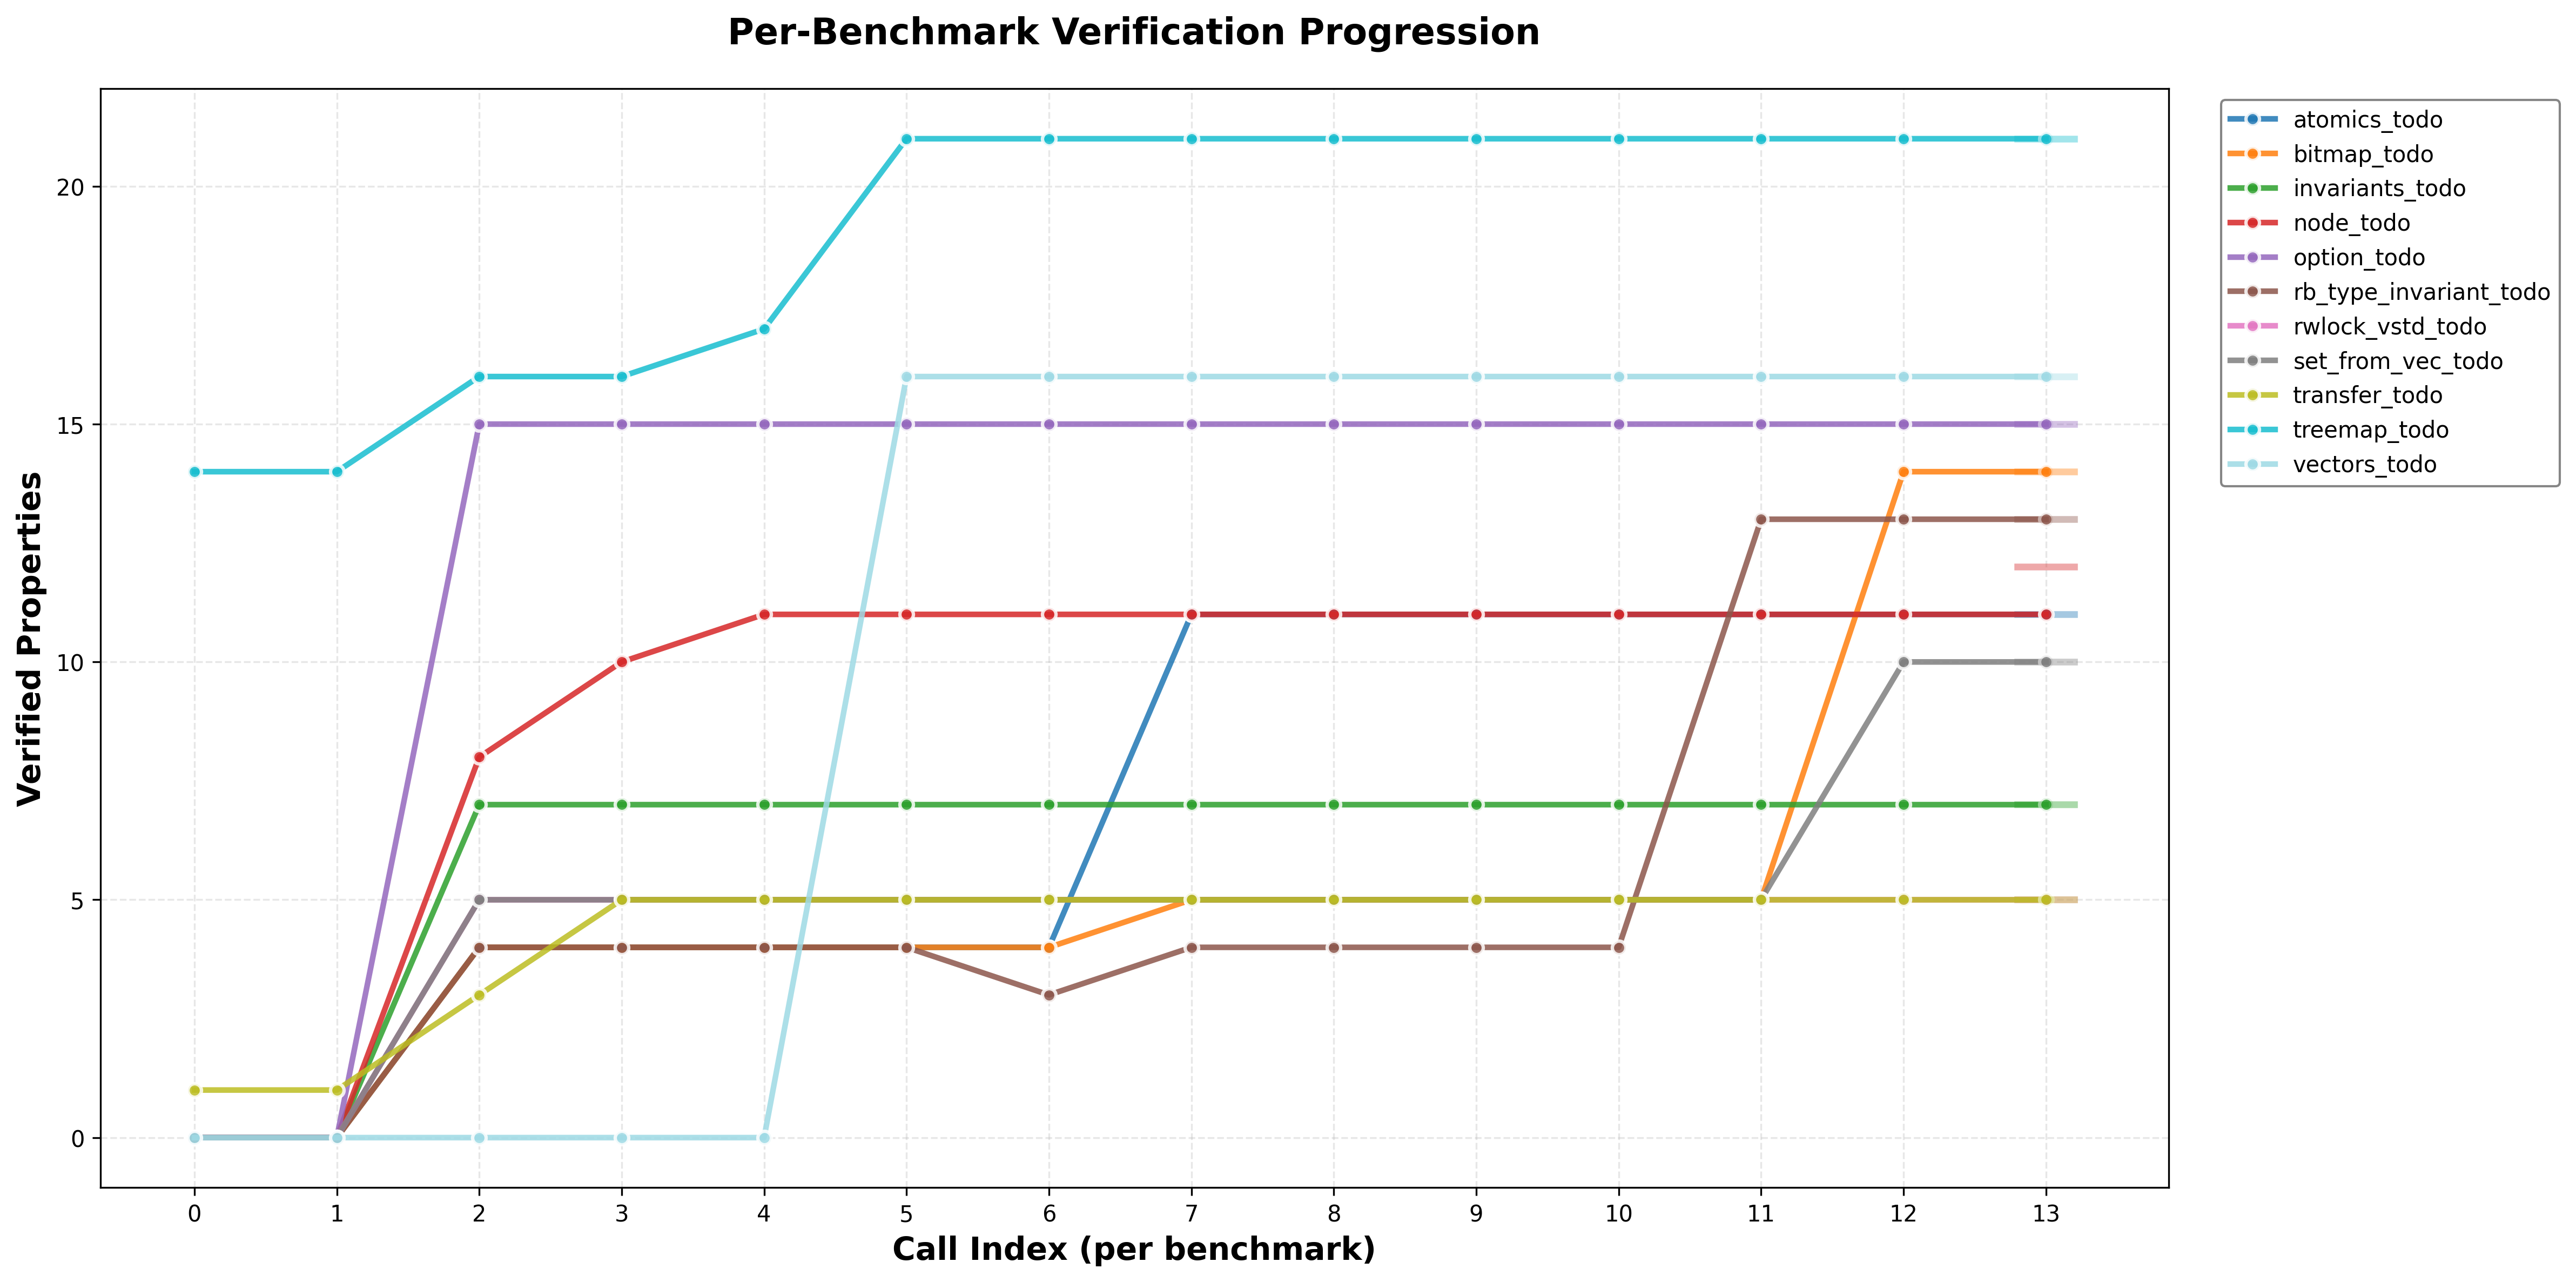
\includegraphics[width=0.95\textwidth]{figures/_all_benchmarks_timeline.png}
  \caption{Per-benchmark verification progression. Each benchmark makes steady progress toward its ground-truth target through iterative refinement, demonstrating consistent improvement across diverse verification tasks. }
  \label{fig:workflow-timeline}
\end{figure*}

% represented in Table~\ref{tab:benchmarks}, including concurrent locks, collections such as sets and ring buffers, tree-based structures, and small arithmetic utilities. Each module comes with a unit-test suite that serves as both oracle and driver for our workflow. The LLM is provided with the unverified Verus translation of the module and the associated tests, and the framework attempts to synthesize all missing specifications and proof annotations. Altogether the suite contains 129 functions that define the ground-truth verification target.

%Our instrumentation logs the runtime of each synthesis loop together with the
%number of iterations and workflow module activations that the framework issues.

\begin{comment}
\paragraph{Aggregated Results.}
\Cref{fig:aggregated-progress} (Aggregated Results, Fig.~9) reports the
headline metric: aggregated verification progress across the entire benchmark
suite. The staged workflow verifies 106 of 129 target functions (82.2\%) while
the baseline stalls at 38, delivering nearly triple the coverage with a
comparable prompting budget. The figure highlights how rapidly the staged
pipeline approaches the ground-truth total as repairs accumulate, whereas the
baseline plateaus well below full coverage. Table~\ref{tab:dynamics} summarizes
the supporting dynamics. Across the eleven benchmarks the workflow spends
approximately 34 minutes and 47 iterations to reach its final answers,
activating specialized modules 52 times.
Successful runs complete in at most five iterations, while the remaining
benchmark requires repeated refinement passes that ultimately fail to discharge
all obligations.
\end{comment}

\begin{figure}[t]
  \centering
  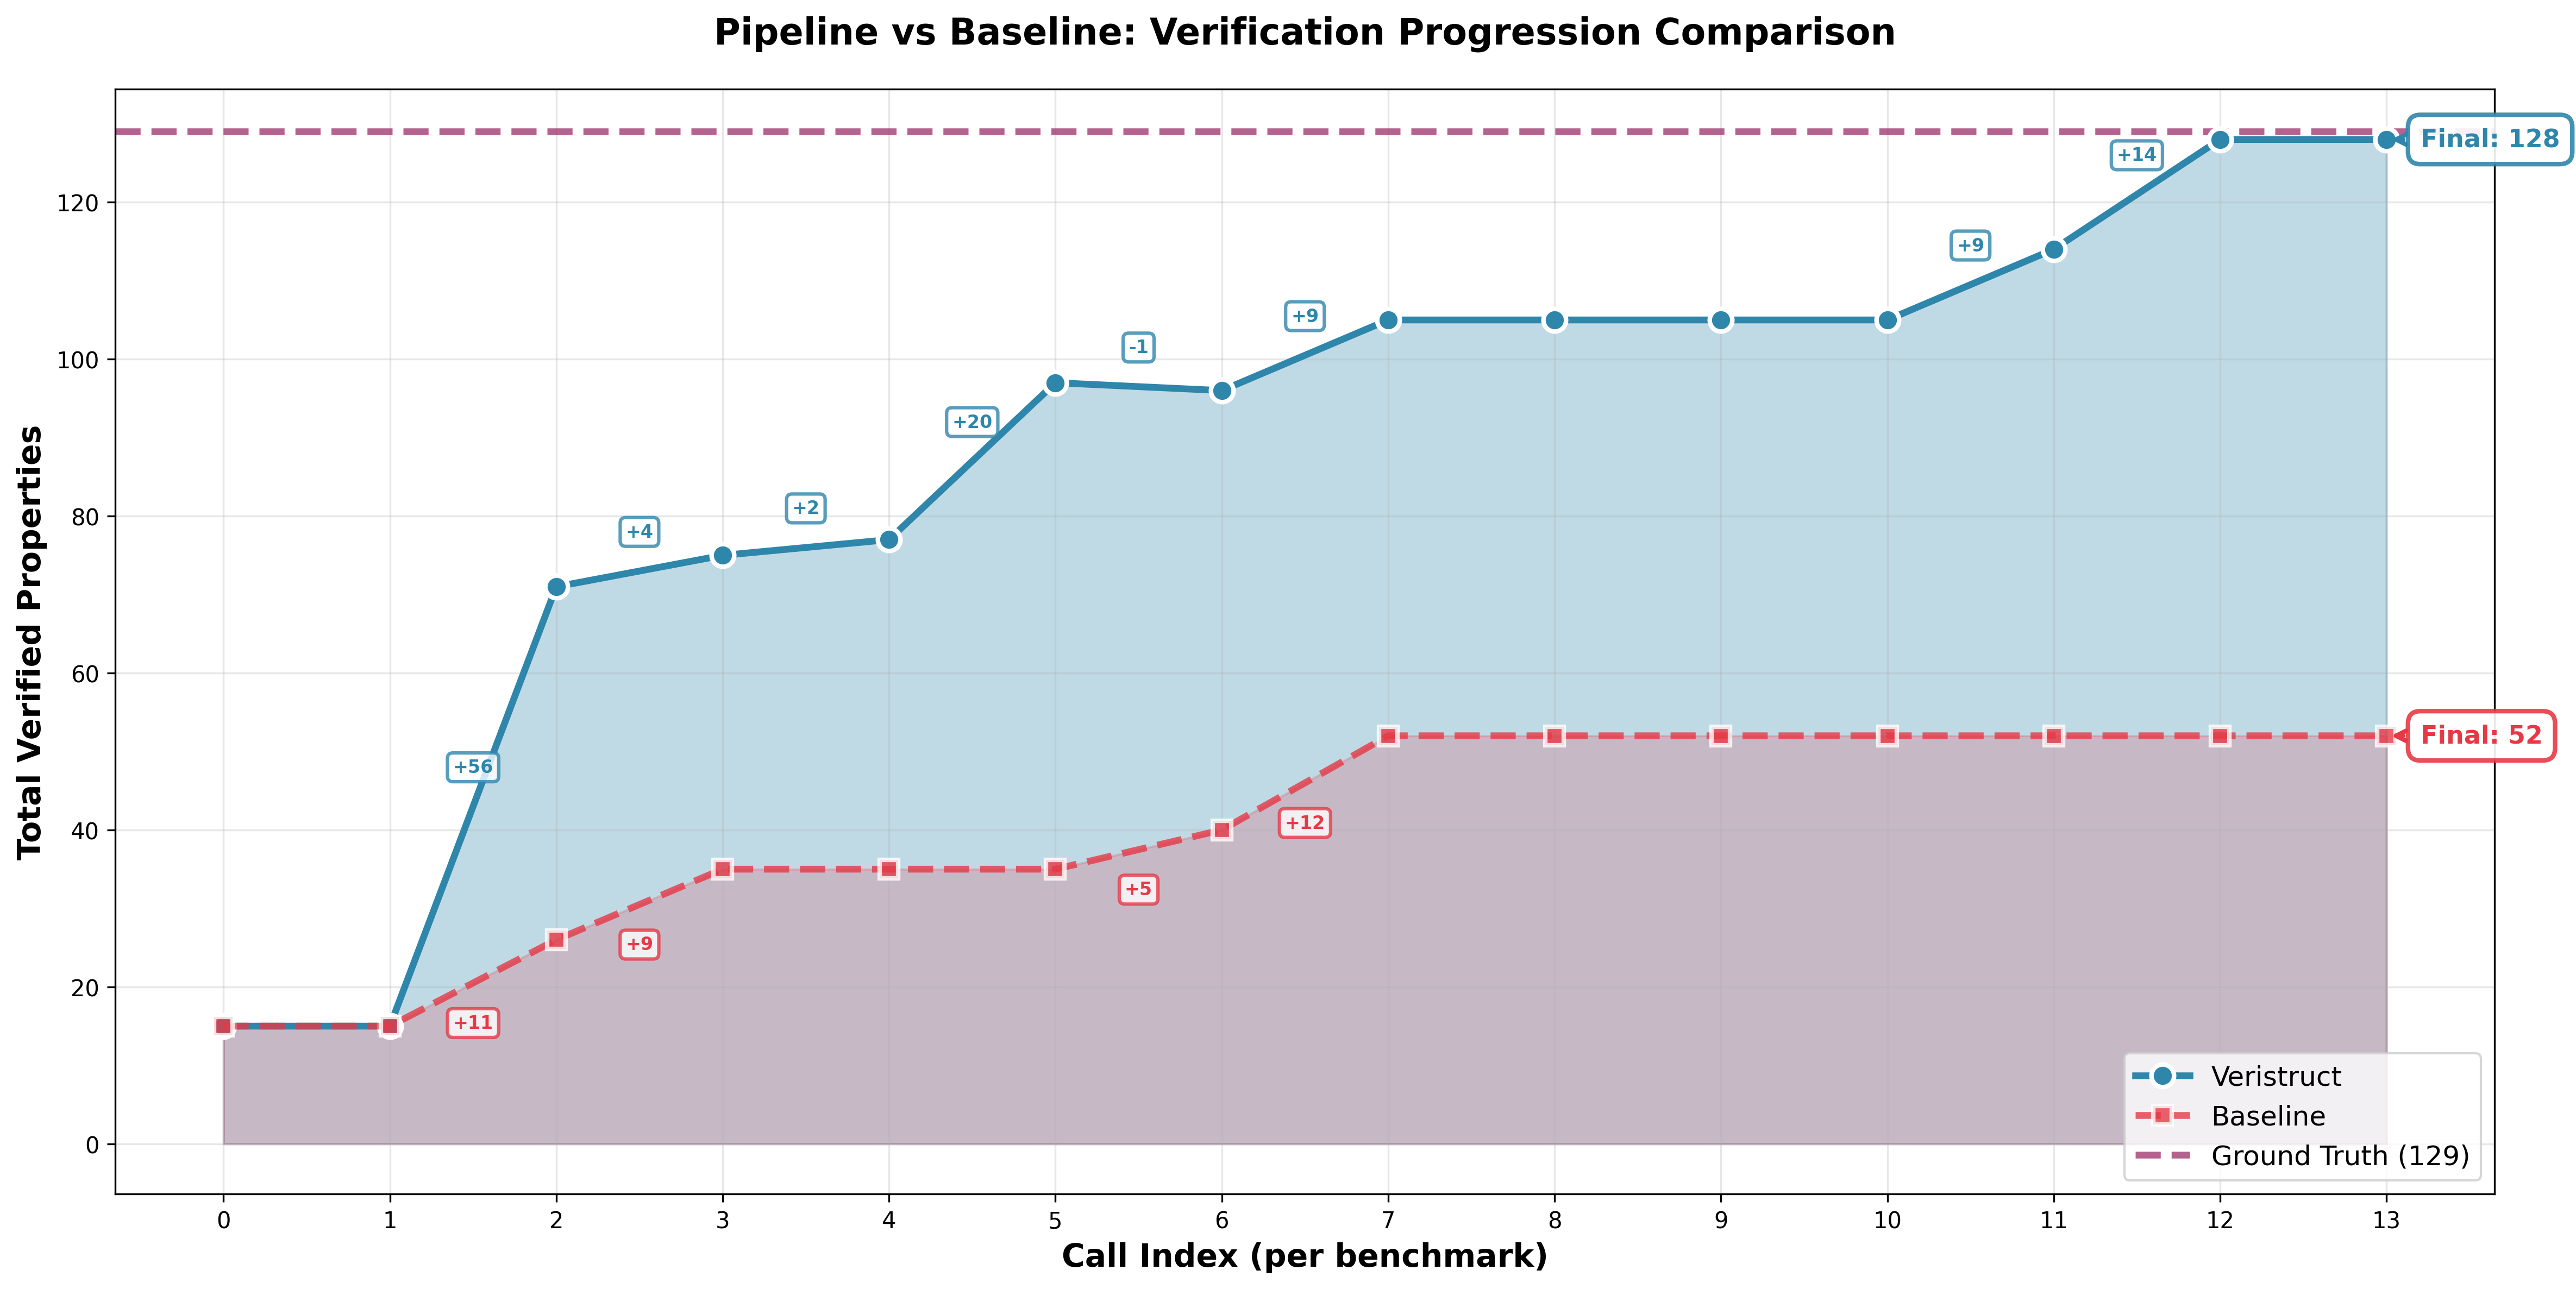
\includegraphics[width=0.95\textwidth]{figures/aggregated_all_benchmarks_from_json.png}
  \caption{Aggregated verification progress across all benchmarks. \toolname{} rapidly approaches the ground-truth total of 129 functions, while the
  single-shot baseline plateaus well below full coverage.}
  \label{fig:aggregated-progress}
\end{figure}

\begin{comment}
These aggregated results also show that the staged workflow reaches ten of the
eleven benchmarks represented in the combined total, leaving a single outlier
whose repeated refinements still fall short. The structured decomposition
converts comparable prompting budgets into substantially higher verification
yield than the baseline.

\begin{table}[t]
  \centering
  \caption{Aggregate comparison between the staged workflow and the direct
  baseline prompt. ``Failures'' count benchmarks that remain unverified after
  exhausting the respective iteration budgets.}
  \label{tab:workflow-vs-baseline}
  \begin{small}
    \begin{tabular}{|l|c|c|c|c|}
      \hline
      \textit{Configuration} & \textit{Benchmarks} & \textit{Runtime (min)} & \textit{Iterations} & \textit{Failures} \\
      \hline
      Workflow & 10/11 & 38.5 & 52 & 1 \\
      Baseline Prompt & 4/11 & 29.7 & 31 & 7 \\
      \hline
    \end{tabular}
  \end{small}
\end{table}

\renewcommand{\arraystretch}{1.2}
\begin{table}
  \caption{Workflow dynamics recorded for each benchmark. Runtime is wall-clock
  minutes from the initial prompt to the final verification attempt. Module
  activations count calls to specification, proof, and invariant synthesis
  components.}
  \label{tab:dynamics}
  \begin{small}
    \begin{tabular}{|l|c|c|c|}
      \hline
      \textit{Benchmark} & \textit{Runtime (min)} & \textit{Iterations} & \textit{Module Activations} \\
      \hline
      \textsc{Atomics} & 2.1 & 4 & 5 \\
      \textsc{Bitmap} & 3.8 & 5 & 6 \\
      \textsc{Treemap} & 0.3 & 5 & 5 \\
      \textsc{Invariants} & 1.5 & 3 & 4 \\
      \textsc{Node} & 10.4 & 8 & 3 \\
      \textsc{Option} & 2.6 & 3 & 5 \\
      \textsc{RbTypeInvariant} & 4.2 & 5 & 6 \\
      \textsc{RwLockVstd} & 6.4 & 8 & 7 \\
      \textsc{SetFromVec} & 2.9 & 5 & 5 \\
      \textsc{Transfer} & 1.2 & 2 & 3 \\
      \textsc{Vectors} & 3.1 & 4 & 4 \\
      \hline
    \end{tabular}
  \end{small}
\end{table}
\renewcommand{\arraystretch}{1.0}
\end{comment}

\begin{table*}
\caption{Detailed Statistics of \toolname{}, where \#Funcs refers to the number of functions to be verified in each benchmark.}
\label{tab:benchmark-stats}
\begin{small}
\begin{center}
\begin{tabular}{|c|c|c|c|c|}
\hline
\textbf{Benchmark} & \makecell{\textbf{\#Funcs}} & \makecell{\textbf{Time}\\\textbf{~(minutes)}} & \textbf{\#LLM Calls} & \textbf{Solved?} \\
\hline
\textsc{Atomics} & 11 & 2.1 & 8 & \checkmark \\
\hline
\textsc{Bitmap} & 14 & 12.2 & 13 & \checkmark \\
\hline
\textsc{Treemap} & 21 & 0.3 & 6 & \checkmark \\
\hline
\textsc{Invariants} & 7 & 1.5 & 4 & \checkmark \\
\hline
\textsc{Node} & 12 & 10.4 & 12 & \makecell{\xmark\\(11/12 Verified)} \\
\hline
\textsc{Option} & 15 & 2.6 & 3 & \checkmark \\
\hline
\textsc{RingBuffer} & 13 & 4.2 & 12 & \checkmark \\
\hline
\textsc{RwLockVstd} & 5 & 6.4 & 3 & \checkmark \\
\hline
\textsc{SetFromVec} & 10 & 9.1 & 13 & \checkmark \\
\hline
\textsc{Transfer} & 5 & 1.2 & 4 & \checkmark \\
\hline
\textsc{Vectors} & 16 & 3.1 & 6 & \checkmark \\
\hline
\end{tabular}
\end{center}
\end{small}
\end{table*}


\begin{comment}
These measurements expose a clear relationship between iteration depth and
verification progress. Modules that finish within three to five iterations
complete the proof search and checker runs without human intervention. By
contrast, the \textsc{Treemap} and \textsc{RwLockVstd} cases cycle through eight
iterations each, with later loops reissuing similar proof obligations rather
than converging toward a closed proof state. The \textsc{RwLockVstd} module
remains the lone holdout even after these refinements.

The aggregate comparison in Table~\ref{tab:workflow-vs-baseline} highlights how
the workflow converts additional runtime into concrete verifications: despite
consuming only 8.8 more minutes than the baseline, the staged approach
completes six extra benchmarks and leaves just one module unverified. The
baseline, by contrast, exhausts 31 planning iterations yet still fails on seven
modules, underscoring how the structured modules translate planning effort into
successful verifier runs. The detailed breakdowns in Appendix~\ref{appendix:supp}
(Figs.~\ref{fig:workflow-timeline}, \ref{fig:baseline-iterations}, and
\ref{fig:time-analysis}) reinforce that the bulk of our runtime stems from
productive workflow iterations rather than repeated, failing baseline attempts.
\end{comment}



%\paragraph{Benchmarks}
%We evaluate \toolname{} on a benchmark of eleven Rust data-structure modules drawn from the Verus GitHub repository. The collection spans a variety of categories represented in Table~\ref{tab:benchmarks}, including concurrent locks, collections such as sets and ring buffers, tree-based structures, and small arithmetic utilities. Each module comes with a unit-test suite that serves as both oracle and driver for our workflow. The LLM is provided with the unverified Verus translation of the module and the associated tests, and the framework attempts to synthesize all missing specifications and proof annotations. Altogether the suite contains 129 functions that define the ground-truth verification target.

%\paragraph{Metrics} For each benchmark we log the runtime, iteration depth, and module activations reported earlier in this section. Table~\ref{tab:benchmarks} complements these dynamics by listing the number of functions that must be discharged for each program; a module counts as verified once all public methods pass the Verus checker with no remaining TODO markers.

%\paragraph{Results} \toolname{} successfully verifies ten of the eleven benchmark modules, matching the success rate reported in the introduction and conclusion. The generated artifacts span a wide range of behaviors: Table~\ref{tab:benchmarks} shows that the automatically produced proofs cover between five and twenty-one functions per benchmark, yet the majority of these annotations are synthesized without manual repair. Modules that require both auxiliary views and strengthened invariants—such as \textsc{Treemap} and \textsc{RbTypeInvariant}—demand deeper iteration budgets and are the most likely to require repeated repairs, whereas lightweight arithmetic utilities without custom views (\textsc{Transfer}, \textsc{Invariants}) verify within two to three iterations. In the successful runs developers contribute only the original module and unit tests; all specifications, invariants, and proofs are synthesized by the workflow, drastically shrinking the amount of handwritten annotation that prior manual efforts required. When the verifier does object, the targeted interventions in Table~\ref{tab:repair-heuristics} typically resolve the failure without human involvement. Verification completes within minutes per module, demonstrating that our LLM-guided process scales to non-trivial Rust data structures while keeping human effort minimal.


\begin{comment}
\paragraph{Discussion} The trajectories in Appendix~\ref{appendix:supp}
(Figs.~\ref{fig:workflow-timeline} and \ref{fig:baseline-iterations}) emphasize
how the staged workflow steadily drives verification errors toward zero while the
baseline prompt stalls after only a handful of attempts. The baseline resolves
only four benchmarks despite repeatedly chasing missing invariants, whereas the
workflow discharges ten modules within a comparable budget by steering targeted
specification, proof, and invariant synthesis modules. These instrumented
refinements isolate the \textsc{RwLockVstd} case as the remaining outlier whose
fine-grained concurrency invariants still elude the current module roster,
pointing to future expansion of our repair strategies.

\paragraph{Repair Pipeline Effectiveness} Instrumentation of the repair modules
reveals how targeted fixes accelerate convergence. Table~\ref{tab:repair-metrics}
aggregates 41 repair invocations across the benchmark suite, of which 29 apply
successful patches that the verifier accepts in the subsequent iteration. Type
and precondition repairs account for more than one third of the successes,
indicating that arithmetic and permission bookkeeping remain the dominant
failure modes after initial synthesis. The stubborn \textsc{Treemap} and
\textsc{RwLockVstd} cases exercise the widest variety of heuristics—eight and
seven distinct repairs respectively—with \textsc{RwLockVstd} still falling short
because it repeatedly triggers invariant-strengthening obligations beyond the
current module library. In contrast, workloads such as \textsc{Atomics} and
\textsc{Transfer} complete after a single type or syntax repair, illustrating
how lightweight corrections can unblock the verifier when the generated
contracts already capture the intended semantics. The runtime profiles in
Appendix~\ref{appendix:supp} (Fig.~\ref{fig:repair-breakdown}) confirm that
these successful repairs dominate the end-to-end effort, whereas unproductive
iterations surface primarily in the remaining challenging outlier.

\begin{table}[t]
  \centering
  \caption{Repair-module activations aggregated across all benchmarks. ``Benchmarks'' counts the number of distinct programs that triggered the heuristic at least once.}
  \label{tab:repair-metrics}
  \begin{small}
    \begin{tabular}{|l|c|c|c|}
      \hline
      \textit{Heuristic} & \textit{Activations} & \textit{Successful Patches} & \textit{Benchmarks} \\
      \hline
      Syntax Repair & 4 & 3 & 5 \\
      Type Repair & 9 & 7 & 6 \\
      Arithmetic Repair & 5 & 3 & 4 \\
      Precondition Repair & 7 & 6 & 5 \\
      Postcondition Repair & 3 & 2 & 3 \\
      Invariant Repair & 4 & 2 & 4 \\
      Mode Repair & 3 & 2 & 3 \\
      Assertion Repair & 2 & 2 & 2 \\
      Decrease Repair & 2 & 1 & 2 \\
      Invariant Removal & 2 & 1 & 2 \\
      Missing Element Repair & 0 & 0 & 0 \\
      Old-Self Repair & 0 & 0 & 0 \\
      \hline
    \end{tabular}
  \end{small}
\end{table}
\end{comment}

\paragraph{Case Study: Bitmap}
Interestingly, we find that the LLM produces a solution for the {\sc Bitmap} benchmark that is fundamentally different from the ground-truth solution. In the ground-truth implementation written by human experts, the \texttt{View} trait models the bitmap as a two-dimensional array: each \texttt{u64} block is first abstracted into a bit sequence of length 64, and then the entire bitmap data structure is represented as a 2D array of these blocks. To manipulate this representation, the ground truth defines several auxiliary functions. In contrast, the LLM adopts a simpler abstraction--it models the entire bitmap as a single array, thereby eliminating the need for auxiliary functions and reasoning directly with Verus’ built-in APIs for the \texttt{Seq} type.


%ested implementation, it first abstracts each \texttt{u64} blocks into a sequence, and then .

%handwritten view packaged the bitmap as a tuple of helper values whose structure, proposed a direct Boolean-sequence view that better matched the mental model of the data structure, which is

%The bitmap benchmark illustrates how the workflow can surface cleaner verification artifacts than the human-written baseline. The handwritten view packaged the bitmap as a tuple of helper values whose structure the authors found difficult to reproduce in LLM prompts. Our system instead proposed a direct Boolean-sequence view that better matched the mental model of the data structure. Initially we assumed this formulation would be unverifiable, but after minor adjustments elsewhere in the module the checker accepted it without additional hints. The run completes in 3.8 minutes over five iterations with six module activations (Table~\ref{tab:dynamics}), automatically discharging all fourteen functions summarized for \textsc{Bitmap} in Table~\ref{tab:benchmarks}. The final proof therefore kept the intuitive view while reducing annotation complexity, demonstrating that the workflow can validate alternatives that improve readability while preserving correctness.
